\chapter{Network I/O Contention}\label{chapter:network}

\section{Throughput Contention}
\subsection{Throughput}
For network I/O stress, we used iPerf3 \cite{iperf}, a tool that benchmarks network 
bandwidth. It supports multiple protocols and can measure TCP, UDP, and SCTP 
throughput. iPerf3 probes the maximum achievable network bandwidth by transmitting a large number 
of packets until reaching the thoughput's upper bound. The tool requires two nodes — a 
server and a client. In our experiments, we measured the 
maximum UDP throughput between clients and servers. We made this choice in order to avoid congestion 
effects introduced by TCP congestion control, which can reduce measured throughput even
when additional bandwidth is available. \\
To quantify throughput degradation caused by contention between the different tenants, 
we conducted the following experiment. \\
\begin{figure}[H]
  \centering
  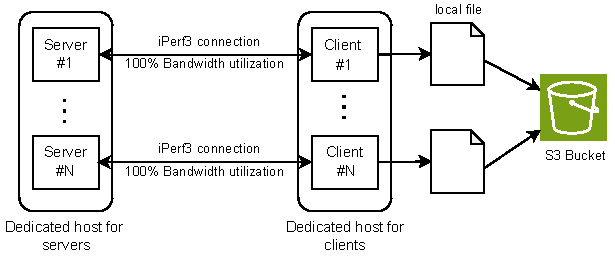
\includegraphics[width=14.5cm, height=6.25cm]{figures/netexp}
  \caption{Throughput contention experiment}
  \label{fig:netexp}
\end{figure}
\noindent
We deployed two dedicated hosts: one to host all the iPerf3 client instances and the other hosting all 
corresponding server instances.
We incrementally add client nodes that are fully utilizing their bandwidth 
through an iPerf3 connection with their paired server. Each client is continuously recording its measured 
throughput to a local log file. we implemeted a python script to compute the average of the 20 recent data 
points in the log file and append the result to a different output file. 
After each client is added, the script is executed across all the client nodes leveraging the distexprunner 
tool. At the end of the experiment, all the output files from the clients are uploaded to an S3 bucket 
for further analysis. \\
In the iPerf3 command executed on the client, we set the duration (using the \texttt{-t} option) 
to 3600 seconds to ensure steady-state network performance without fluctuations caused by calling 
the command multiple times. \\
All the VMs were provisioned in the same availability zone and resided
in the same Virtual Private Cloud as mentioned in the \nameref{chapter:infra} chapter. 

\subsection{m5 family}
Unlike other resources such as CPU and RAM, which are statically divided between the different tenants 
based on instance type, network bandwidth is shared among the different co-tenants without a fix
specification of the expected bandwidth per tenant. Typically, for instances with 16 vCPUs or less, 
AWS specifies the bandwidth upper bound, e.g., "Up to 10 Gbps" \cite{network_bandwidth}. However these 
instances still have a baseline bandwidth. A network I/O credit mechanism is employed that 
allows the instance to use burst bandwidth for a short period of time, ranging from 5 to 60 minutes,
depending on the instance type \cite{network_bandwidth}. \\ 
We'll analyze throughput contention on instances belonging to the m5 family. Key
performance metrics for the m5 dedicated host can be found in Table \ref{tab:dedicated-hosts}.
Table \ref{tab:m5_spec} depicts the most important network related specifications for the different 
instance types.
\begin{table}[H]
\centering
\begin{tabular}{lccc}
\toprule
\textbf{Type} & \textbf{vCPUs} & \textbf{Burst BW (Gbps) \cite{cloudspecs}} & \textbf{Baseline BW \cite{cloudspecs}} \\
\midrule
m5.large     & 2  & 10 & 0.75 \\
m5.xlarge    & 4  & 10 & 1.25 \\
m5.2xlarge   & 8  & 10 & 2.5  \\
m5.4xlarge   & 16 & 10 & 5    \\
m5.8xlarge   & 36 & 10 & 10   \\
m5.12xlarge  & 72 & 12 & 12   \\
m5.metal     & 96 & 25 & 25   \\
\bottomrule
\end{tabular}
\caption{Specifications of m5 Instance Types (BW = Bandwidth)}
\label{tab:m5_spec}
\end{table}
\noindent
For single flow traffic, the maximum burst bandwidth of 10 Gbps is only attainable when the the client and 
the server reside in the same cluster group. For instances who are not in the same cluster group, single flow 
traffic is limited to 5 Gbps \cite{network_bandwidth}.  The clients and the servers 
can't be in the same cluster groups since they are in different dedicated hosts. This means that the 
single-flow traffic between the client and the servers is limited to 5 Gbps. To bypass this restriction, 
we create two client connections, that can be achieved using the P option in the iPerf3 tool. \\
Bandwidth throttling for smaller instances takes at least 5 minutes to take effect, during which the instance
has access to 10 Gbps burst bandwidth. We conduct our experiments in this time window. It is particularly 
interesting to observe the extent of the network degradation in comparison to the baseline bandwidth 
for each instance size. The first experiment features the m5.4xlarge instance type, 
of which the dedicated host can accomoadate 6. To provide a better 
visualization of the results, we present each node in an independent graph.
\begin{figure}[H]
\centering
\begin{tikzpicture}
\begin{groupplot}[
    group style={
        group size= 2 by 4,
        horizontal sep=1.25cm,
        vertical sep=1.25cm,
        xlabels at= edge bottom,
        ylabels at=edge left,
    },
    width=6cm,
    height=4cm,
    xlabel={Number of Nodes},
    ylabel={Throughput},
    title style={yshift=-1ex},
    ymin=2, ymax=10,
    xtick distance = 1, 
    xmin=0,
    grid=both,
]

% Node 1
\nextgroupplot[title={Node 1}]
\addplot[mark=*, blue, thick] coordinates {(0,9.96)(1,9.96) (2,8.06)(3,5.97) (4,4.90) (5, 4.01)};

% Node 2
\nextgroupplot[title={Node 2},]
\addplot[mark=square*, red, thick] coordinates {(1,9.96) (2,7.83)(3,5.97) (4,4.98) (5, 4.17)};
% Node 3
\nextgroupplot[title={Node 3}]
\addplot[mark=triangle*, green, thick] coordinates {(2,8.00) (3,5.98) (4,4.91) (5, 4.17)};


\nextgroupplot[title={Node 4}]
\addplot[mark=diamond*, orange, thick] coordinates {(3,5.96) (4, 4.98) (5,3.99)};

% Node 4
\nextgroupplot[title={Node 5}, xlabel={Number of Nodes}]
\addplot[mark=diamond*, orange, thick] coordinates {(4,4.91) (5, 4.11)};

% Node 4
\nextgroupplot[title={Node 6}, xlabel={Number of Nodes}]
\addplot[mark=diamond*, orange, thick] coordinates {(5,4.25)};
\end{groupplot}
\end{tikzpicture}
\caption{UDP Throughput of m5.4xlarge nodes when incrementally increasing the tenants}
\label{fig:boxplot}
\end{figure}

\noindent
As expected, the first and the second clients, when alone on the dedicated host had access to a burst 
bandwidth of 9.96 Gbps. The third tenant caused the average throughput to drop to 7.96 Gbps, while the 
addition of a fourth neighbor further reduced it to 5.96 Gbps. We practically notice no variation between 
the different nodes. The fifth neighbor reduced the throughput of all the co-tenants to practically 
the baseline bandwidth of the m5.4xlarge (5 Gbps) with an average throughput of 4.94 Gbps. The 6th node 
introduced the first significant decrease under the baseline bandwidth to an average of 4.12 Gbps, 
which is 17.6\% less than the baseline bandwidth. Starting from the the 3rd tenant, the sum 
of the throughput across all the nodes is always around 24.7 Gbps.  This was expected as the bandwidth 
of the m5.metal is 25 Gbps, which should represent the upper limit for the sum of the throughputs of all the nodes
residing on the same dedicated host. For the xlarge, 2xlarge, and 4xlarge types, the product of the 
maximum number of the instances on the dedicated host multiplied by the baseline bandwidth of the respective
instance type (5 Gbps) is 30 Gbps, which is 16.7\% smaller than the possible bandwidth of 25 Gbps. 
This explains the average degradation of 17\% we saw in the previous experiment. The same behavior
should be expected when using xlarge and 2xlarge instances. For the large instance type, however, the 
product is equal to
\begin{math} 48 \times 0.75 = 36\end{math} Gbps. 
25 Gbps is 30\% smaller than 36 Gbps. This indicates that a  
degradation of around 30\% is expected when using m5.large instances at full host capacity. 
We verify this assumption in the next experiment. Since the dedicated host can host 48 of m5.large 
instances, we can't individually plot the graph of each instance. We used a plotbox graph to display the 
distribution of the throughputs at the different levels. We also used a step size of 8 neighbors, to be 
able to present the results in one graph. 

\begin{figure}[H]
\centering
\begin{tikzpicture}
\begin{axis}[
    boxplot/draw direction=y,
    ylabel={Throughput},
    xlabel={Number of Nodes},
    xtick={1,2,3,4,5,6, 7, 8},
    xticklabels={8, 16, 24, 32, 40, 48},
    ymin = 0.2,
    ymax = 4,
    width=11cm,
    height=7cm,
    grid = both,
]


%\addplot+[
%    boxplot,
%    draw=black,
%] table[row sep=\\, y index=0] {
%data \\
%9.96 \\ 
%}; 

% Boxplot A
\addplot+[
    boxplot,
    draw=black,
] table[row sep=\\, y index=0] {
data \\
2.19 \\ 2.17 \\ 2.19 \\ 3.19 \\ 3.88 \\ 3.17 \\ 3.87 \\ 3.21 \\
};

% Boxplot B
\addplot+[
    boxplot,
    draw=black,
] table[row sep=\\, y index=0] {
data \\
1.12 \\ 1.12 \\ 1.12 \\ 1.82 \\ 2.03 \\ 1.82 \\ 2.00 \\ 1.80 \\ 
1.12 \\ 1.12 \\ 1.18 \\ 2.13 \\ 1.18 \\ 1.19 \\ 1.12 \\ 1.97 \\
};

% Boxplot C
\addplot+[
    boxplot,
    draw=black,
] table[row sep=\\, y index=0] {
data \\
0.86 \\ 0.86 \\ 0.86 \\ 1.16 \\ 1.21 \\ 1.16 \\ 1.20 \\ 1.14 \\ 
0.86 \\ 0.86 \\ 0.86 \\ 1.25 \\ 0.86 \\ 0.85 \\ 0.86 \\ 1.18 \\ 
0.85 \\ 0.85 \\ 1.14 \\ 0.86 \\ 1.13 \\ 0.86 \\ 0.86 \\ 1.27 \\
};

% Boxplot D
\addplot+[
    boxplot,
    draw=black,
] table[row sep=\\, y index=0] {
data \\
0.75 \\ 0.75 \\ 0.75 \\ 0.75 \\ 0.75 \\ 0.75 \\ 0.75 \\ 0.75 \\ 
0.75 \\ 0.75 \\ 0.75 \\ 0.75 \\ 0.75 \\ 0.75 \\ 0.75 \\ 0.75 \\ 
0.75 \\ 0.75 \\ 0.75 \\ 0.75 \\ 0.75 \\ 0.75 \\ 0.75 \\ 0.75 \\ 
0.75 \\ 0.75 \\ 0.75 \\ 0.75 \\ 0.75 \\ 0.75 \\ 0.75 \\ 0.75 \\
};
% Boxplot E
\addplot+[
    boxplot,
    draw=black,
] table[row sep=\\, y index=0] {
data \\
0.28 \\ 0.28 \\ 0.27 \\ 1.15 \\ 0.84 \\ 0.85 \\ 0.84 \\ 1.10 \\ 
0.31 \\ 0.29 \\ 0.21 \\ 1.14 \\ 0.21 \\ 0.19 \\ 0.31 \\ 0.87 \\ 
1.11 \\ 1.09 \\ 1.22 \\ 1.26 \\ 1.20 \\ 0.29 \\ 1.59 \\ 1.46 \\ 
0.23 \\ 0.20 \\ 0.55 \\ 0.53 \\ 0.44 \\ 0.54 \\ 0.26 \\ 0.52 \\ 
0.26 \\ 0.23 \\ 0.82 \\ 0.78 \\ 0.21 \\ 0.20 \\ 0.22 \\ 0.21 \\
};
% Boxplot F
\addplot+[
    boxplot,
    draw=black,
    solid,
] table[row sep=\\, y index=0] {
data \\
0.70 \\ 0.67 \\ 0.14 \\ 0.98 \\ 0.76 \\ 0.74 \\ 0.59 \\ 0.94 \\ 
0.13 \\ 0.71 \\ 0.28 \\ 0.58 \\ 0.18 \\ 0.17 \\ 0.13 \\ 0.60 \\ 
0.16 \\ 0.19 \\ 0.96 \\ 0.20 \\ 0.97 \\ 0.15 \\ 0.70 \\ 0.89 \\ 
0.19 \\ 0.18 \\ 0.76 \\ 0.89 \\ 0.97 \\ 0.88 \\ 0.72 \\ 0.76 \\ 
0.14 \\ 0.75 \\ 0.62 \\ 0.20 \\ 0.20 \\ 0.18 \\ 0.23 \\ 0.18 \\ 
0.16 \\ 0.57 \\ 0.58 \\ 0.92 \\ 0.75 \\ 0.56 \\ 0.15 \\ 0.58 \\
};
\end{axis}
\end{tikzpicture}
\caption{Throughput (UDP) of m5.large nodes when incrementally increasing the number tenants}
\end{figure}
\noindent
The first node has access to a throughput of 9.96 Gbps, which represents the maximum burst bandwidth. 
At 8 neighbors, the average throughput drops to 3 Gbps. We then observe a gradual degradation 
with an average of 1.5 Gbps at 16 nodes, 1 Gbps at 24 nodes, and  0.75 Gbps at 32 nodes,  which corresponds 
to the baseline bandwidth of the m5.large instance type. 
At this level, we interestingly notice zero variation between the 
different co-tenants. At 40 nodes, the average decreases to 0.614 Gbps and further to 0.51 Gbps at 48 nodes.  
At full capacity, The average throughput (0.51 Gbps) is 30.7\% lower than the baseline bandwidth of the 
m5.large instance (0.75 Gbps). This more significant performance degradation close to 30\% was expected 
as hypothesized earlier. In this experiment, we also observe an important performance variation 
between the different nodes compared to the previous experiment.


\section{Latency}
\subsection{Methodology}
For latency benchmarking, we employed both \textit{iPerf3} and \textit{sockperf} \cite{sockperf}. 
Sockperf is a network benchmarking utility capable of measuring the latency of packets with a 
sub-nanosecond resolution. It introduces minimal overhead by leveraging the Time Stamp Counter (TSC) 
registers that count the number of CPU cycles for measuring latency \cite{sockperf}. 
Sockperf requires a client-server setup as well: the client sends mutliple packets to the server
, receives responses and records the \ac{RTT} for each packet. 
The tool provides different options to visualize the results with varying granularity. 
A CSV file is generated listing the send and response times for each individual packet,
along with a report of the average latency and key metrics such as the 90th and 99th percentile. \\
The objective of the latency experiment was to evaluate the effect of increasing aggregate throughput 
utilization of neighbors on the latency of the test node. The experiment is structured as 
follows.
\begin{figure}[H]
  \centering
  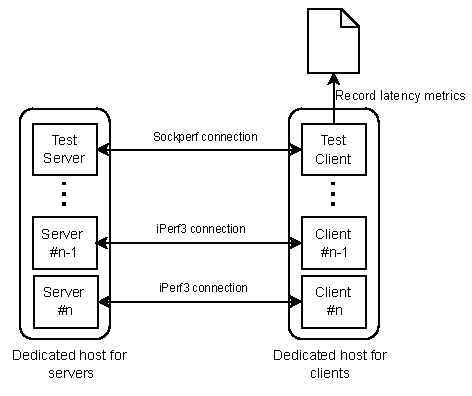
\includegraphics[width=11cm, height=8.5cm]{figures/latexp}
  \caption{Throughput contention experiment}
  \label{fig:latexp}
\end{figure}
\noindent
Similar to the throughput experiment, we deploy two dedicated hosts, 
one hosting all clients and one hosting all servers. Initially, only the client test node 
and its corresponding server are created. We measure the latency between them and record it as a baseline 
value. After that, we deploy all the remaining clients and incrementally increase their aggregate 
throughput usage in 1 Gbit/s steps (or smaller as we notice the presence of latency degrdation).
This is possible through an iPerf3 functionality that allows the specification of an exact throughput 
value for the client, allowing us to control the aggregated throughput of the neighbors.
After each step, i.e. increase, we measure the latency between the test client node and 
the test server using sockperf with the ping-pong option. The results are then recorded locally on the 
client side. 
Since all dedicated hosts, including the client test node and server, are located within 
the same \ac{AZ} (See Chapter \ref{chapter:infra}),
external latency variability is minimized, allowing for a better identification of latency 
degradation caused by increased throughput usage of the neighbors. \\ 
\subsection{m5 family}
We start the first latency experiment using the m5 dedicated host. At each throughput level, we executed 
the sockperf command 30 times and averaged the metrics recorded. Figure \ref{fig::latencym5} provides
the results of the experiment. 
\begin{figure}[H]
\centering
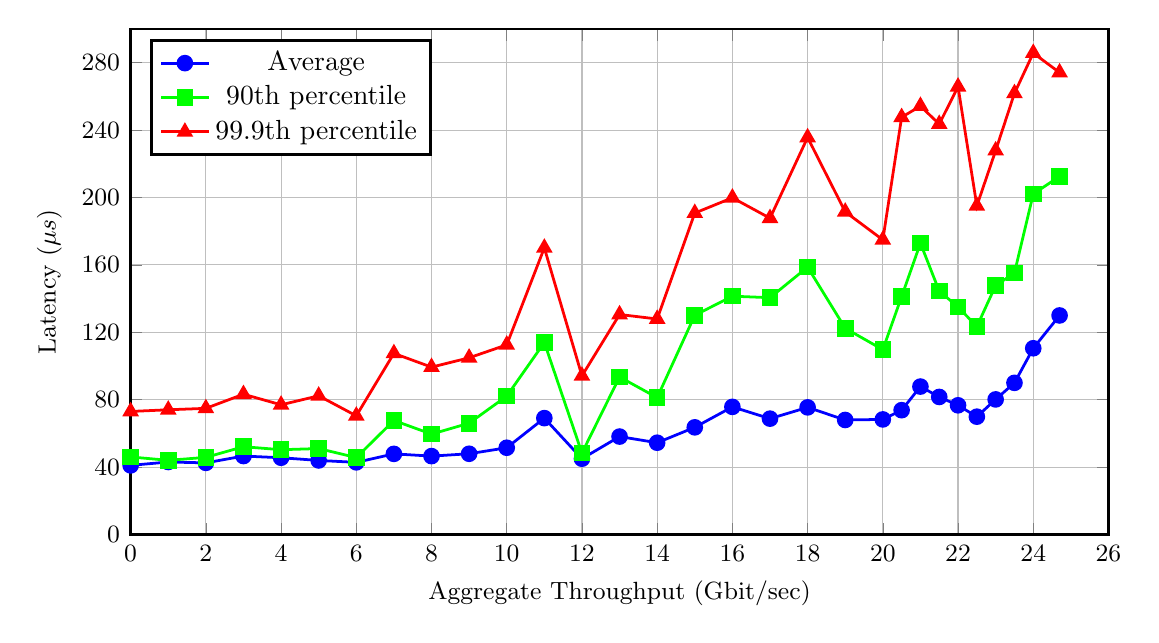
\begin{tikzpicture}
\begin{axis}[
    width=14cm,
    height=8cm,
    xlabel={Aggregate Throughput (Gbit/sec)},
    ylabel={Latency (\(\mu s\))},
    grid=major,
    xmin=0, xmax=26,
    ymin=0, ymax=300,
    xtick={0,2,...,25.5},
    ytick={0,40,80,...,300},
    line width=1pt,
    mark size=2.5pt,
    tick label style={font=\small},
    label style={font=\small},
    legend style={at={(0.02,0.98)},anchor=north west},
    title style={font=\bfseries\small},
]
\addplot[
    mark=*,
    color=blue,
] coordinates {
(0, 41)
(1, 43)
(2, 42.484)
(3, 46.525)
(4, 45.526)
(5, 43.926)
(6, 42.783)
(7, 47.828)
(8, 46.493)
(9, 47.892)
(10, 51.454)
(11, 69.042)
(12, 44.942)
(13, 58.097)
(14, 54.435)
(15, 63.578)
(16, 75.729)
(17, 68.724)
(18, 75.424)
(19, 67.945)
(20, 68.269)
(20.5, 73.756)
(21, 87.778)
(21.5, 81.605)
(22, 76.654)
(22.5, 69.899)
(23, 80.156)
(23.5, 89.978)
(24, 110.510)
(24.7, 129.992)
};
\addlegendentry{Average}

% 90th percentile (2nd value)
\addplot[
    mark=square*,
    color=green,
] coordinates {
(0, 46)
(1, 44)
(2, 45.745)
(3, 52.078)
(4, 50.296)
(5, 50.974)
(6, 45.630)
(7, 67.651)
(8, 59.554)
(9, 66.028)
(10, 82.090)
(11, 113.933)
(12, 48.304)
(13, 93.470)
(14, 81.212)
(15, 130.075)
(16, 141.434)
(17, 140.527)
(18, 158.698)
(19, 122.399)
(20, 109.679)
(20.5, 141.194)
(21, 172.899)
(21.5, 144.428)
(22, 135.069)
(22.5, 123.395)
(23, 147.747)
(23.5, 155.251)
(24, 202.095)
(24.7, 212.558)
};
\addlegendentry{90th percentile}

% 99.9th percentile (3rd value)
\addplot[
    mark=triangle*,
    color=red,
] coordinates {
(0, 73)
(1, 74)
(2, 74.844)
(3, 83.237)
(4, 76.947)
(5, 82.303)
(6, 70.414)
(7, 107.474)
(8, 99.315)
(9, 104.859)
(10, 112.546)
(11, 170.118)
(12, 94.143)
(13, 130.557)
(14, 127.888)
(15, 190.757)
(16, 199.854)
(17, 187.725)
(18, 235.632)
(19, 191.516)
(20, 174.864)
(20.5, 247.645)
(21, 254.280)
(21.5, 243.589)
(22, 265.750)
(22.5, 195.045)
(23, 227.853)
(23.5, 261.827)
(24, 285.742)
(24.7, 274.180)
};
\addlegendentry{99.9th percentile}
\end{axis}
\end{tikzpicture}
\caption{Average Latency vs Bandwidth}
\label{fig::latencym5}
\end{figure}
\noindent
The baseline average latency between the test client and the server was 41 \(\mu s\), which is 
relatively low considering that both reside in the same \ac{AZ}. 
From the start of the experiment up to an aggregate throughput of 9 Gbit/s, latency exhibited 
only minor degradation, increasing by 11.9\% to 47 \(\mu s\).
Beyond this point, latency began to rise significantly in a gradual manner that became sharper,
as the aggregate throughput approached the maximum aggregate throughput of 24.7 Gbit/s. 
It increased from 51 \(\mu s\) at 10 Gbit/s to 130 \(\mu s\) at 24.7 Gbit/s , corresponding to an 155\%
increase. Overall, the experiment revealed a total latency degradation of approximately 217\%, 
a substantial value that could have severe implications for latency-sensitive workloads. \\ 
Furthermore, the results also indicate siginificant variability. 
The 90th percentile latency values were, on average, 41 \(\mu s\) higher than the 
mean, while the 99.9th-percentile values exceeded the mean by 100  \(\mu s\), on average. 
This variability became more pronounced as the mean latency degraded. Figure \ref{fig:sub} illustrates 
the difference between the mean and the 90th-percentile latency value, clearly highlighting 
the increased variability with increased aggregate throughput. 

\begin{figure}[H]
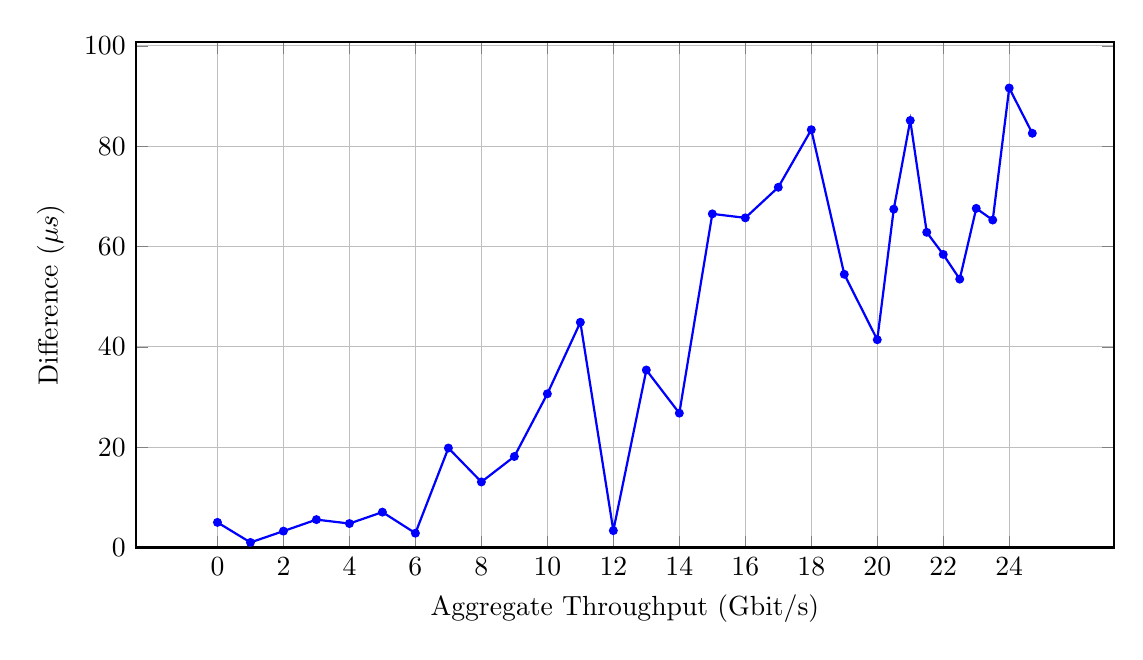
\begin{tikzpicture}
\begin{axis}[
    width=14cm,
    height=8cm,
    grid=major,
    xlabel={Aggregate Throughput (Gbit/s)},
    ylabel={Difference (\(\mu s\))},
    ymin=0,
    xtick={0,2,4,6,8,10,12,14,16,18,20,22,24},
    ytick distance=20,
    thick,
    legend style={at={(0.98,0.02)},anchor=south east}
]

\addplot[
    blue,
    mark=*,
    mark options={scale=0.6},
] coordinates {
(0, 5.000)
(1, 1.000)
(2, 3.261)
(3, 5.553)
(4, 4.770)
(5, 7.048)
(6, 2.847)
(7, 19.823)
(8, 13.061)
(9, 18.136)
(10, 30.636)
(11, 44.891)
(12, 3.362)
(13, 35.373)
(14, 26.777)
(15, 66.497)
(16, 65.705)
(17, 71.803)
(18, 83.274)
(19, 54.454)
(20, 41.410)
(20.5, 67.438)
(21, 85.121)
(21.5, 62.823)
(22, 58.415)
(22.5, 53.496)
(23, 67.591)
(23.5, 65.273)
(24, 91.585)
(24.7, 82.566)
};
\end{axis}
\end{tikzpicture}
\caption{Difference between the 90th-percentile latency values and the mean}
\label{fig:sub}
\end{figure}


\newpage
\section{Discussion}
For throughput, we found out that the (average) maximum degradation for any instance type 
can be approximated by the following formula. The bandwidth of the physical server is equal
to the bandwidth of the metal instance of the concerned family (if it's offered):
\[
\frac{\text{Bandwidth of physical server / Maximum number of nodes}}
     {\text{Baseline Bandwidth of the instance type}} \times 100
\]

\noindent
For all the instance types belonging to the m5 family except the large type, the maximum degradation 
relative to the baseline bandwidth is roughly 17\%, whereas for the large type it reaches 30\%. In 
their work, Loyd et. al \cite{characterizing_public}, found similar results using the m5d dedicated host,
which is similar to the m5 host, as they both have the same processor and number of vCPUs.  
For large instances, they observed a normalized performance degrdation equal to 94.6\% due to VM 
co-location. However this percentage is relative to the inital throughput of the first m5d.large, 
i.e., the burst bandwidth of 10 Gbps. It implies that the  average throughput at the end was 0.54 Gbit/s, 
very close to the results presented in Figure \ref{fig:boxplot}. Lloyd et. al also found
that degradation tends to increase with successive  VM generation, which can be explained by 
denser and larger physical servers capable of hosting an increasing number of tenants. \\ 
For latency, We measured an average degradation of 217\% with increasing aggregate throughput of the 
neighbors. We used the m5.4xlarge instance for our experiment. However, the results 
should be independent of the instance type, as the only influential factor is the aggregate 
throughput of the neighboring nodes. It's important to note that the datapoints exhibited 
very high variability and the results can significantly different between different runs. 
The percentile values, increasingly far from the mean, support this. 

